
\documentclass[12pt,a4paper]{report}

\title{Proyecto de modelización - Programación evolutiva\\ \textbf{El problema de balanceo de líneas de montaje}} 
\author{Paul Rohel - Alejandro Regidor Orellana}
\date{\today}

\usepackage[spanish]{babel}
\usepackage[utf8]{inputenc}
\usepackage[T1]{fontenc}
\usepackage{graphicx}
\usepackage{mathtools, amsfonts, amssymb, amsthm}
\usepackage{float}
\usepackage[margin=2.5cm]{geometry} 
\usepackage[hidelinks]{hyperref}
\usepackage[T1]{fontenc}
\usepackage{lmodern}
\usepackage{xcolor} 
\setlength{\parskip}{10pt}
\renewcommand{\chaptername}{}

\setlength{\parindent}{0pt}

\makeatletter
\renewcommand{\@makechapterhead}[1]{\vspace*{50\p@}%
  \begin{center}%
    {\normalfont\huge\bfseries #1\par}%
  \end{center}\vskip 40\p@}
\makeatother

\begin{document}

\maketitle
\tableofcontents

\chapter{Introduccion}
\section{Panteamiento del problema}
El problema de balanceo de líneas de ensamblaje puede plantearse de diferentes maneras. Dadas $n$ tareas, cada una con un tiempo de procesamiento asignado y una lista de relaciones de precedencia entre ellas, dichas tareas deben asignarse a $m \leq n$ estaciones de trabajo.

Una de las variantes clásicas, conocida como \texttt{Simple Assembly Line Balancing Problem tipo 1} (SALBP-1), consiste en encontrar una asignación de las $n$ tareas a las estaciones de manera que se minimice el número de estaciones, dado un tiempo de ciclo preestablecido.

En cambio, la variante sobre la que hemos trabajado (SALBP-2) tiene como objetivo encontrar una asignación de tareas que minimice el tiempo de ciclo, dado un número fijo de estaciones $m$. En este contexto, el tiempo de ciclo se define como el tiempo total más largo asignado a una estación, es decir, el máximo entre todas las estaciones.

\section{Objetivos}
El principal objetivo de este trabajo fue profundizar en los algoritmos genéticos, y no solo desde un punto de vista teórico, sino también desde uno práctico, aplicando este tipo de algoritmos a un problema real.\\
Concretamente, se buscó modelizar el problema SALBP-2, explorando cómo representar las soluciones, definir operadores genéticos efectivos y adecuarse a las restricciones específicas del dominio del problema.\\
A través de este proceso, se trató de comprender mejor la capacidad y las limitaciones de usar este tipo de metodología en contextos aplicados, así como desarrollar habilidades para el diseño e implementación de este tipo de algoritmos.

\section{Presentación general del algoritmo genético}

Para resolver este problema, implementamos un algoritmo genético. 
Dadas $n$ tareas que deben asignarse a $m$ estaciones, el espacio de búsqueda contiene $O\left(\binom{n}{m}\right)$ soluciones posibles. 
Una solución, es decir, una asignación de las tareas entre las diferentes estaciones, se codifica posicionalmente como un lista unidimensional indexada de $0$ a $n-1$, 
cuyos elementos toman valores enteros entre $0$ y $m-1$. Por ejemplo, la lista $[0, 0, 0, 1, 0, 2, 2, 1]$ representa una solución para un problema con $8$ tareas distribuidas en $3$ estaciones.

Para codificar las relaciones de precedencia entre las tareas, utilizamos una matriz $A$ de tamaño $n \times n$ definida de la siguiente manera:

$
\forall i,j \in \{0,\dots,n-1\},$
$
A(i,j) = 
\begin{cases}
1 & \text{si la tarea } j \text{ precede directamente a la tarea } i \\
0 & \text{en caso contrario}
\end{cases}
$


Dado que todas las tareas que deben preceder a otra deben asignarse a una estación anterior o, como máximo, a la misma estación que la tarea que las sigue, 
las relaciones de precedencia imponen restricciones estrictas sobre la validez de las soluciones. También es necesario verificar que exactamente todos los grupos dados, y solo esos, aparezcan en los valores de la lista solución.

La función de evaluación de un individuo consiste, esencialmente, en devolver el mayor tiempo entre estaciones. Por lo tanto, el objetivo del problema es encontrar el individuo que minimice dicha función, penalizando a aquellos que no cumplen con las restricciones previamente establecidas.

La principal dificultad que enfrentamos en este trabajo fue la gestión de la diversidad de los individuos: encontrar un equilibrio entre una selección demasiado estricta, que conduce a una convergencia hacia un mínimo local, y una selección demasiado permisiva, que favorece en exceso la generación de individuos no válidos.

Hemos decidido codificar la totalidad del problema sin utilizar bibliotecas específicamente dedicadas a los algoritmos genéticos. Dada la relativa complejidad del problema, especialmente en lo que respecta a la modelización de las restricciones de precedencia, resultó más sencillo partir desde cero que intentar adaptar funciones pensadas para estructuras más simples.

Elegimos programar en Python, ya que este lenguaje resulta relativamente más cómodo en términos de indexación de matrices y gestión de memoria que lenguajes como Ada o C. La variedad de herramientas y bibliotecas disponibles en Python, junto con su buena documentación, también nos permitió resolver aspectos particulares como la generación de grafos para representar las soluciones, o el cálculo automático del orden topológico.


\chapter{Proceso de creación y evolución del algoritmo}

\section{Generación de una población inicial}

Una población inicial es generada por la función \texttt{población inicial}. Una población consiste simplemente en un lista de soluciones, cuya dimensión está determinada por el parámetro $dim\_pob$.

\subsection*{Generar individuos aleatorios}

Para llenar una población, nuestro primer enfoque fue generar individuos completamente aleatorios, sin tener cuenta de las restricciones. Suponíamos que, dado que nuestra función de evaluación penalizaba con un valor arbitrariamente alto a los individuos no válidos, acabaríamos, tras algunas generaciones, con una población compuesta mayoritariamente por individuos válidos.

Sin embargo, las restricciones del problema son tan estrictas que, incluso con grafos de apenas $6$ tareas con tiempos relativamente equilibrados y distribuidas en $3$ estaciones, obteníamos poblaciones con un $90\%$ de individuos no válidos.
Esta minoría de individuos válidos no era suficiente para permitir que el algoritmo avanzara hacia algún punto estacionario.

\subsection*{Generar individuos aleatorios hasta que cumplen las restricciones}

Nuestro segundo enfoque consistió entonces en seguir generando individuos completamente aleatorios, hasta que cumplieran con las restricciones del problema, para luego añadirlos a la población.\\

La verificación de las restricciones está a cargo de la función booleana \texttt{condiciones}, que devuelve falso si un individuo \texttt{sec} no contiene exactamente —y únicamente— valores entre $0$ y $m-1$, o si existe una relación de precedencia directa entre dos estaciones, especificada en la matriz correspondiente \textit{A}, que no se respeta en el individuo. Es decir, si:
\[
\exists i,j \in \{0,\dots,n-1\} \text{ tal que } A(i,j) = 1 \text{ y } sec[i] < sec[j]
\]

Sin embargo, el principal defecto de este enfoque se hizo evidente muy rápidamente: se necesitaba un número extremadamente alto de iteraciones para generar siquiera un solo individuo válido para la población.
El algoritmo resultaba entonces especialmente lento, al punto de no llegar siquiera a completar la primera generación.

\subsection*{Generar individuos mediante orden topológico}

Con el fin de generar individuos con mayor probabilidad de cumplir con todas las restricciones, utilizamos la noción de orden topológico: un orden lineal —entre varios posibles— de los nodos de un grafo dirigido acíclico, representado en nuestro caso por la matriz de precedencia $A$. 

Utilizamos la función \texttt{topological\_sort} de la biblioteca \texttt{networkx} para extraer un orden topológico del grafo derivado de $A$ (véase la función \texttt{matriz\_a\_lista\_adyacencia}).

De hecho, para cada individuo, la primera tarea en el orden topológico se asigna a la última estación $m-1$. Luego, para cada tarea siguiente ($ord\_top[i]$), se elige aleatoriamente (mediante \texttt{random.randint()}) una estación en función de la tarea anterior ($ord\_top[i-1]$), de manera que no comience después que esta: la misma estación o la inmediatamente anterior.

Este enfoque nos permitió obtener un primer algoritmo funcional, pero presenta una limitación importante relacionada con la sobrecarga de la estación $0$.

En efecto, durante la construcción de un individuo, la probabilidad de asignar una estación anterior con respecto a la tarea precedente es del $50\%$. Esto provoca un descenso rápido hacia la estación $0$, donde ya no es posible asignar estaciones más bajas. Como resultado, las tareas siguientes tienden a acumularse en dicha estación.

Como resultado, nos enfrentamos a un problema de convergencia prematura. Todas las soluciones generadas eran muy similares entre sí, presentando sistemáticamente la sobrecarga de la estación $0$, y el algoritmo exploraba únicamente una porción muy limitada del espacio de soluciones posibles.


\subsection*{Uniformización de la distribución de las estaciones}

Con el fin de paliar la sobrecarga de la primera estación, reemplazamos el muestreo equiprobable mediante $random.randint()$ por un muestreo que permite uniformizar al máximo la distribución de las tareas entre las estaciones.

Durante la generación de un individuo siguiendo un orden topológico, la probabilidad de que una tarea pertenezca a la estación anterior a la de la tarea precedente es $p$; la probabilidad de que pertenezca a la misma estación es $0.99 - p$; y la de que pertenezca a la estación siguiente es $0.01$.\\ 
 
Después de varias pruebas, vimos que el valor óptimo de $p$ no puede determinarse de forma arbitraria y que debe calcularse en función del número de estaciones y de tareas del problema (ver archivo $bestp.py$).

Este tipo de estructura es conocido como Cadena de Márkov, y en nuestro caso por no variar $p$, homogénea. Queríamos encontrar un $p$ tal que la distribución de las tareas en cada una de las $m$ estaciones fuera uniforme.

Simulamos a traves de un proceso de fuerza bruta en el que para cada $p\in[\frac1 {10},\frac 1 2]$ con pasos de $0.01$ se simulan $n$ cadenas de Márkov, y se estima la frecuencia con la que se ocupa cada posición. Luego se calcula el error cuadrático medio respecto a una cadena completamente uniforme y así obteniendo el mejor valor de $p$ que hace mas uniforme la cadena.

\subsection*{Combinación de los modos de generación}

Aunque el modelo de generación de individuos siguiendo un orden topológico ahora sea uniforme, este sigue llevando a un estancamiento del algoritmo en un mínimo local.

Para introducir una mayor diversidad a lo largo de las generaciones, decidimos generar una parte de la población de forma completamente aleatoria, sin restricciones. Tras varias pruebas, parece que la proporción óptima entre individuos generados por ambos modos es del $50\%$.

Asociado a una función de evaluación que asigna una puntuación no arbitraria a los individuos no válidos, el algoritmo se acerca más a la solución exacta del problema. Para una cantidad de individuos generados inferior al $10\%$ del tamaño del espacio de búsqueda en el caso de los grafos más pequeños, o incluso al $10\,000\%$ para los más grandes, la solución calculada presenta un tiempo de ciclo que, en la mayoría de los casos, se sitúa alrededor de un $5\%$ por encima del valor de la solución óptima.

La incorporación de una variación aleatoria de los órdenes topológicos extraídos de $A$ en el modelo no parece ser particularmente eficaz, ya que conduce a resultados que no son mejores.

\section{Función de evaluación}

La función de evaluación \texttt{score} está definida por:

\[
score(\text{individuo}) = 0.6 \cdot \text{tiempo de ciclo} + 0.2 \cdot \text{dispersión} + 0.1 \cdot \text{n\_fallos} \cdot \text{media}
\]
\vspace{0.5cm}

con:

\begin{itemize}
\item tiempo de ciclo : el tiempo máximo asignado a una estación.
\item dispersión : una medida del equilibrio del tiempo entre las estaciones,
igual a la diferencia entre el tiempo de ciclo y el tiempo mínimo asignado a una estación.
\item $\text{n\_fallos}$ : el número de tareas que no respetan las restricciones del problema.
\item media : el promedio de los tiempos entre las estaciones.
\end{itemize}

El ajuste de los coeficientes asociados a los términos de la función se determinó empíricamente. Asociados a nuestros mecanismos de selección y generación de la población inicial, permiten que el algoritmo avance lo más lejos posible hacia la solución exacta del problema.

El peso asociado al tiempo de ciclo es el más alto, ya que es precisamente esta medida la que nos interesa en este problema y que buscamos minimizar.

Decidimos integrar una medida del equilibrio de los tiempos entre las estaciones (la dispersión) por dos razones:
\begin{itemize}
    \item La primera es que, al inicio de nuestro trabajo, debido a una mala interpretación del problema, definimos nuestra función de evaluación únicamente como una medida de equilibrio. Sin embargo, decidimos que resultaba relativamente eficaz, contribuyendo a la minimización del tiempo de ciclo.
    \item La segunda razón es que la inclusión de esta segunda medida permite valorar ciertos individuos portadores de estructuras potencialmente favorables para la reducción del tiempo de ciclo, aunque este último los penalice. Esto contribuye a favorecer la diversidad de los individuos válidos, una característica que buscamos maximizar para que el algoritmo no se estanque en un mínimo local.
\end{itemize}



El término de penalización para los individuos no válidos ($\text{n\_fallos} \cdot \text{media}$) permite favorecer a aquellos individuos no válidos que violan menos restricciones en comparación con aquellos que las violan en mayor medida. Esto permite discriminar razonablemente entre individuos válidos y no válidos, al mismo tiempo que permite la reproducción de individuos que no necesariamente siguen el orden topológico definido durante la generación de la población.

Hemos elegido multiplicar el número de violaciones de las restricciones por la media de los tiempos de las estaciones, con el fin de obtener un término de penalización que se ajuste proporcionalmente a la escala de cada grafo considerado.

\section{Selección, recombinación y reproducción}

Los módulos de selección, recombinación y reproducción están implementados mediante una única función: \texttt{seleccion}. En esta sección, se presenta el mecanismo que ha demostrado el mejor rendimiento tras la experimentación, tras haberlo enfrentado a otros métodos de selección como por ejemplo torneo.

\subsection{Selección}

En cada generación, se conserva el mejor individuo sin aplicarle ninguna transformación. Este individuo se determina mediante una ordenación basada en el valor de su puntuación (\texttt{clasificación}). Esta forma de elitismo garantiza que la mejor solución encontrada no empeore con el paso de las generaciones.\\

Para determinar qué individuos se reproducen entre los individuos restantes, utilizamos una selección por torneo, en la que se elige un solo individuo entre cuatro seleccionados al azar (\texttt{class\_torneo}). Este método permite la reproducción de individuos potencialmente nuevos por completo, generados en la generación anterior, lo que favorece la introducción de diversidad genética. Sin embargo, para mantener una presión selectiva que favorezca a los individuos con mejor desempeño —a menudo resultado de cruces anteriores—, hemos optado por comparar grupos de cuatro individuos a la vez.  Este enfoque logra un equilibrio entre diversidad y velocidad de convergencia.\\

También probamos la selección por ruleta (\texttt{class\_rueda}). Esta selección adopta la forma de una nueva ordenación, esta vez de tipo probabilístico. El peso de cada individuo se calcula como la diferencia entre su puntuación y la puntuación máxima entre los individuos comparados. La función \texttt{random.sample()} permite realizar automáticamente un muestreo sin reemplazo, normalizado en función de estos pesos. Los individuos seleccionados se añaden uno a uno a una nueva subpoblación.\\
Sin embargo, esta selección resulta menos eficaz que la selección por torneo, ya que es más elitista: los individuos con mayor probabilidad de ser elegidos tienden a ser siempre los mismos, lo que provoca una estancación más rápida del algoritmo.


\subsection{Recombinación}

Una vez conservado el mejor individuo y el resto ordenado mediante selección por ruleta, aplicamos las siguientes transformaciones: el primer tercio de la población se cruza y los individuos hijos reemplazan a los dos primeros tercios de la población; el último tercio se regenera utilizando \texttt{poblacion\_inicial}.
Posteriormente, se aplica una operación de mutación a todos los individuos, con excepción del mejor.

Las proporciones mencionadas se determinaron experimentalmente. Se ha comprobado que un equilibrio entre población reproducida y población regenerada es el más eficaz: si la proporción de individuos reproducidos es demasiado alta, la diversidad se reduce en exceso; mientras que si la proporción de individuos regenerados es demasiado elevada, la diversidad se vuelve excesiva y el algoritmo no converge hacia una solución válida.

\subsection{Reproducción}
Se consideraron dos tipos de operadores de cruce: el cruce en dos puntos y el cruce uniforme.

Durante una primera parte de nuestra experimentación se utilizó un operador de cruce en dos puntos. Este tipo de cruce parecía, en teoría, mas eficaz, ya que tendía a conservar la estructura de los individuos validos. Sin embargo, tras hacer comparaciones entre ambos métodos, lo que inicialmente parecía una ventaja resulto contraproducente: ya que al conservar tanto la estructura, se reducía drásticamente la variabilidad de las soluciones. Y por esta razón, se optó finalmente por el uso de un cruce uniforme.

En concreto, utilizamos un cruce semi-uniforme. Entre los individuos seleccionados, elegimos aleatoriamente dos individuos sin reemplazo ($cruce$). A partir del intercambio de $k$ genes seleccionados aleatoriamente siguiendo el orden topológico, se generan cuatro individuos hijos (\texttt{cruce2a2uniforme}).

Aunque pueda parecer contraintuitivo, conservar cuatro hijos por cruce, reduciendo así a la mitad el número de cruces, resulta más eficaz que conservar solo dos y permitir que todos los individuos se reproduzcan. Podemos suponer que, en este caso, la diversidad depende más de la variedad dentro de la descendencia que del número de individuos que participan en la reproducción.\\
De hecho, tras un cierto número de generaciones, los individuos que logran reproducirse tienden a parecerse cada vez más entre sí, mientras que los generados aleatoriamente presentan puntuaciones generalmente mucho más bajas, al no beneficiarse de la adaptación acumulada. Por ello, resulta más interesante generar más variedad a partir de una fracción reducida de una población que se ha vuelto muy homogénea.

Las restricciones del problema son tan estrictas que un cruce completamente uniforme no resulta efectivo: casi todos los individuos generados por dicho cruce son inválidos.\\

Este cruce resulta muy eficaz si, y sólo si, el número \(k\) de genes a intercambiar está adecuadamente ajustado al grafo considerado. No hemos encontrado una función satisfactoria que relacione \(k\) con las características del grafo, ya sea en términos de dimensiones (\(m\), \(n\)) o de complejidad (medidas de convergencia o divergencia del grafo de precedencias, número total de relaciones de precedencia).\\
Dado que sabemos que el algoritmo converge en pocas iteraciones (del orden de un centenar) y sin una fase prolongada de estancamiento hacia una solución muy cercana a la óptima cuando el parámetro \(k\) está bien ajustado, hemos optado por el siguiente enfoque. Inicialmente fijamos \(k = 1\), y cuando la solución permanece sin cambios durante más de 20 generaciones, aumentamos \(k\) en 2 y regeneramos completamente la población. Este método implica, por lo tanto, una reinicialización completa del algoritmo. Sin embargo, dado el número relativamente bajo de iteraciones necesarias para evaluar si el valor de \(k\) es adecuado, esta estrategia resulta  viable.

Por supuesto, hasta alcanzar el número de generaciones definido por el usuario, almacenamos por separado el mejor individuo obtenido en cada reinicialización. Al final, el algoritmo devuelve la mejor de las soluciones entre todas las almacenadas.


\subsection{Mutación}

Aplicamos un único tipo de mutación que consiste en mover aleatoriamente una tarea a una estación adyacente. Aplicada a toda la población excepto al mejor individuo, esta mutación permite no aumentar significativamente el número de individuos inválidos.\\
Las mutaciones más pronunciadas, como el intercambio aleatorio de estaciones entre dos tareas, alteran demasiado la estructura de los individuos.
\chapter{Experimentación}
\section{Datos usados en la experimentación}
\label{section:Datos}
Durante la experimentación, hemos usado tres tipos distintos de datos en los que probar nuestro algoritmo genético: problemas simples generados manualmente, problemas aleatorios y \textit{data-sets}.\\
Al comienzo de nuestra experimentación, al comenzar desde cero, nuestro algoritmo genético no era capaz de encontrar soluciones en un tiempo razonable, por lo que decidimos generar manualmente problemas pequeños en los que comprobar si estaba funcionando nuestro algoritmo.\\
De ahí pasamos a incrementar poco a poco el tamaño de los problemas para probar cómo escalaba, hasta un punto en el que era inviable crear problemas manualmente, por lo que recurrimos a la generación aleatoria de problemas. Este tipo de datos fue útil para comprobar que nuestro algoritmo era capaz de encontrar mejores soluciones.\\
Sin embargo, una vez el algoritmo ya era estable, el no tener soluciones con las que comparar nuestros resultados era insuficiente para sacar conclusiones, por lo que pasamos al tercer y último método: los \textit{data-sets}.\\
En concreto, usamos los datos de la página \textcolor{blue}{\href{https://assembly-line-balancing.de/salbp/benchmark-data-sets-1993/}{assembly-line-balancing.de}}, de donde obtuvimos el \textit{data-set} de Scholl, que contiene datos acerca de varios grafos SALBP y soluciones analíticas para nuestro caso, SALBP-2. Por lo tanto, el resto de la experimentación y resultados, los cuales fueron los más significativos, se realizaron usando este \textit{data-set} como referencia.
\newpage
\section{Metodología}
    En cuanto a la metodología, por lo general ha sido prueba y error. Dividimos algoritmo en distintas partes e íbamos probando cada opción que teníamos para ver cual es la que mejor resultados alcanzaba.
    Este tipo de pruebas al principio era suficiente fijándose en las soluciones, sin embargo, a medida que se hacia mas complejo el algoritmo decidimos introducir dos partes claves en como se ha desarrollado el algoritmo:
    \begin{itemize}
        \item \textbf{Visualización del grafo solución en tiempo real.}, debido a que no eramos capaces de procesar que pasaba a lo largo de las generaciones mirando las soluciones en forma de listas, decidimos implementar una función que dibujara el grafo solución correspondiente con cada nueva mejor solución. Esta visualización nos ayudó a entender mejor el comportamiento del algoritmo a lo largo del tiempo y nos permitió identificar problemas como la endogamia, la poca diversidad en las poblaciones iniciales, el estancamiento en soluciones subóptimas, entre otros.
        \item \textbf{Gráficas sobre las puntuaciones}, aunque con el dibujo del grafo era suficiente para encontrar problemas graves hubo otros aspectos más sutiles —como la comparación entre distintos métodos de selección, cruce y mutación—, que podian analizarse solo con las soluciones o el grafo. Por esta razón, también utilizamos gráficas que muestran la evolución de la puntuación a lo largo de las generaciones. Estas representaciones nos ayudaron a comprender mejor el comportamiento del algoritmo y elegir esta combinación de selección, recombinación y reproducción, después de comparar varios métodos distintos.
    \end{itemize}
    \begin{figure}[H]
    \centering
    \begin{minipage}{0.48\textwidth}
        \centering
        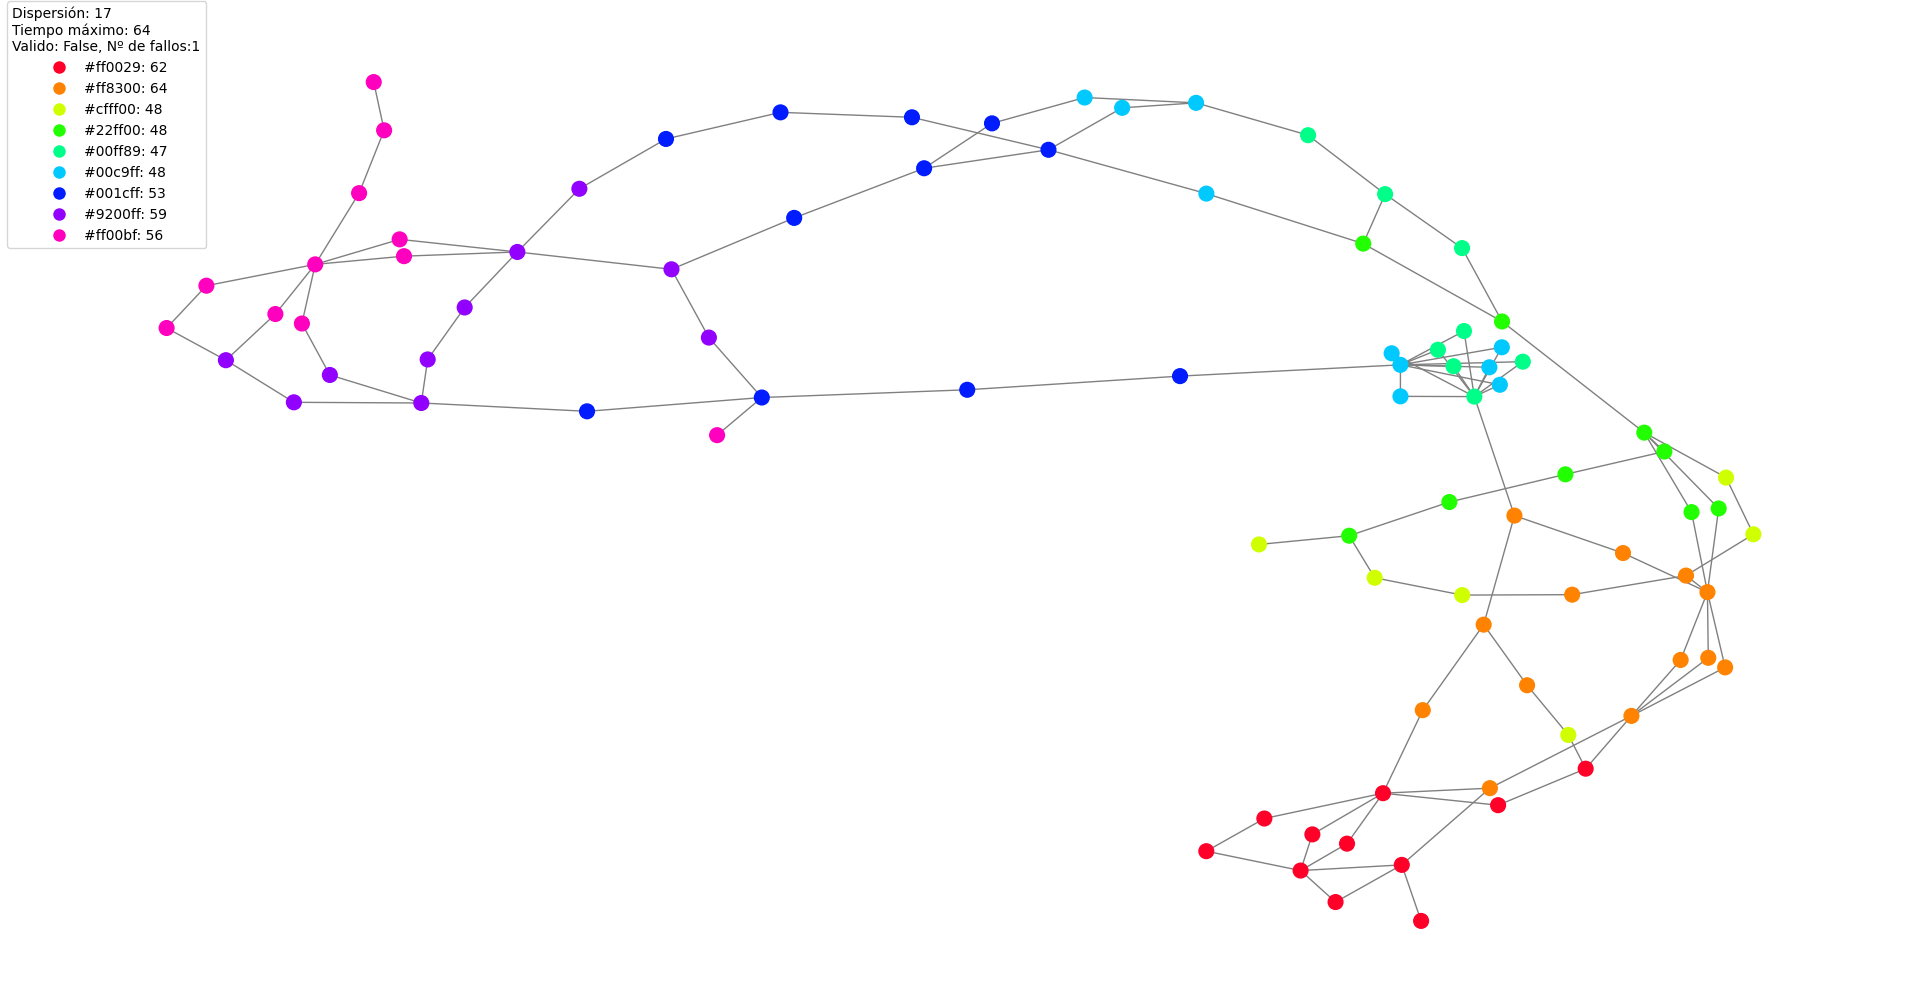
\includegraphics[width=\linewidth]{DATA/grafo_lutz2.png}
        \caption{Grafo de una solución}
        \label{fig:figura1}
    \end{minipage}\hfill
    \begin{minipage}{0.48\textwidth}
        \centering
        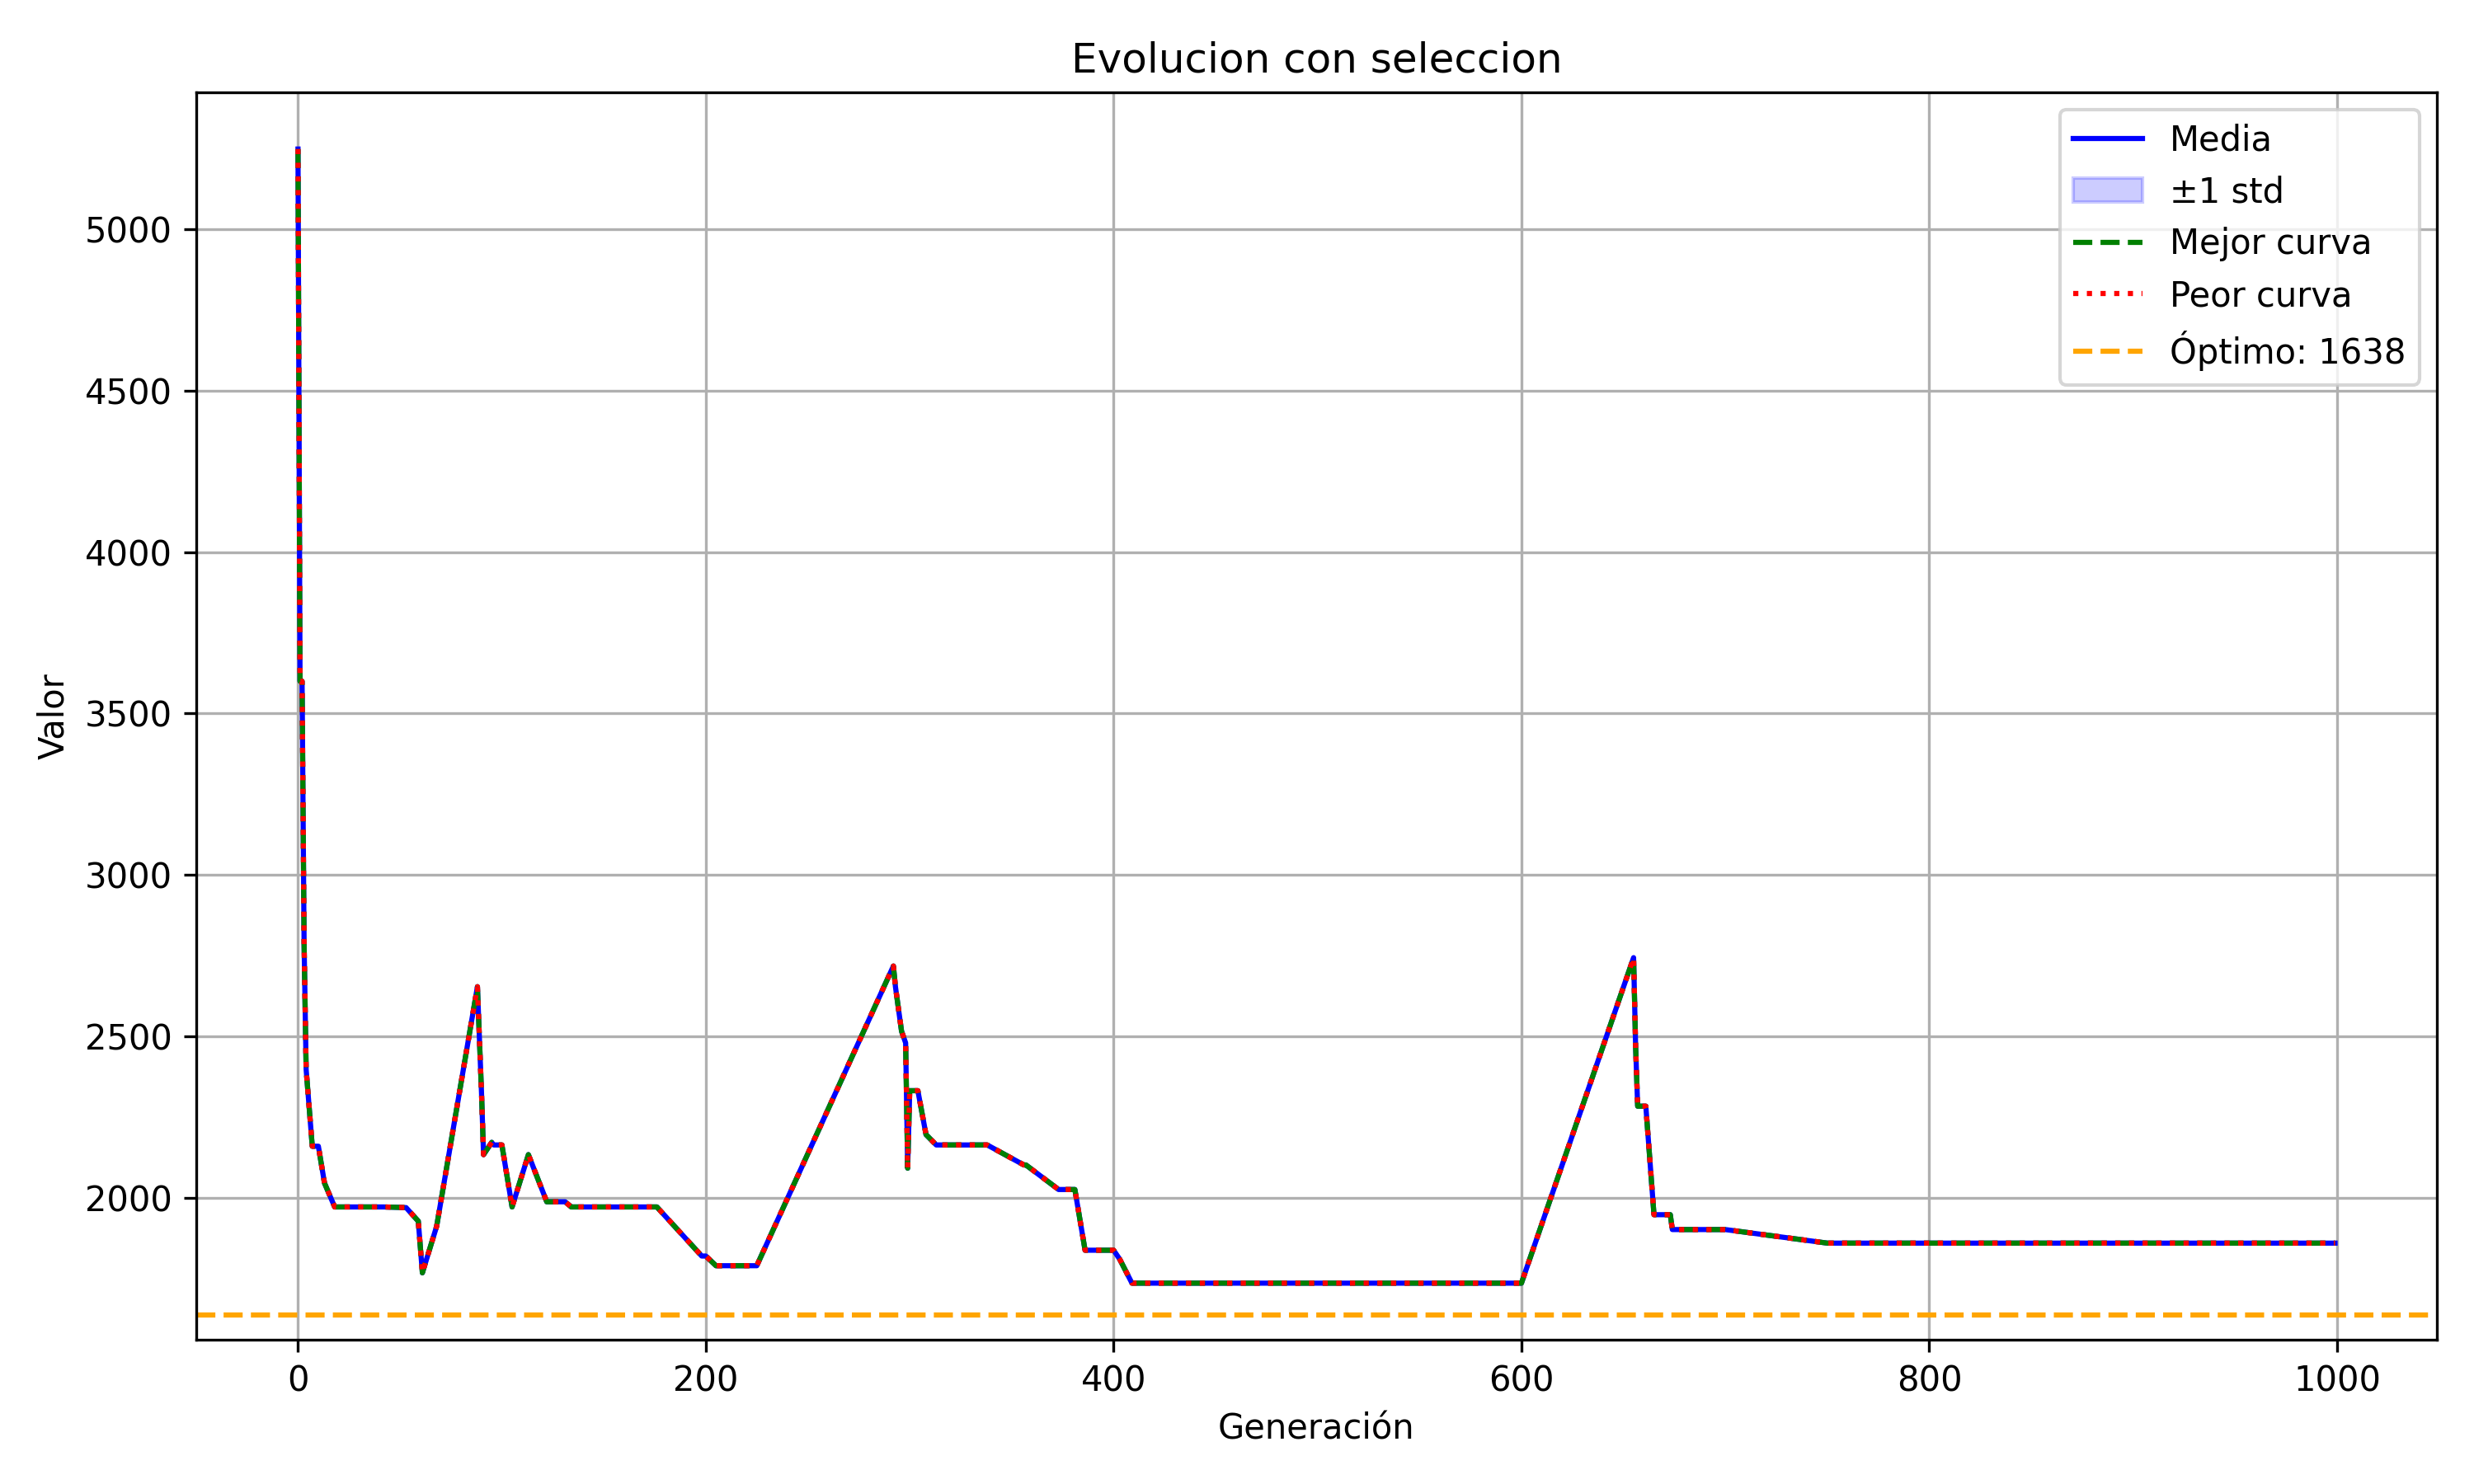
\includegraphics[width=\linewidth]{DATA/lutz1_M9.png}
        \caption{Grafico sobre las soluciones de lutz1 con numero de estaciones, $m=9$}
        \label{fig:figura2}
    \end{minipage}
\end{figure}
\chapter{Resultados y conclusión}
\section{Resultados experimentales}

Para evaluar el rendimiento del algoritmo genético propuesto, se realizaron experimentos sobre distintas instancias del problema SALBP-2. Las pruebas se centraron en analizar la calidad de las soluciones obtenidas, la estabilidad del algoritmo y el impacto de diferentes configuraciones de operadores genéticos (selección, cruce y mutación).

A lo largo de las iteraciones del algoritmo, se observó una mejora progresiva en las soluciones. En la Figura~\ref{fig:evolucion-punt} se presenta la evolución de la puntuación promedio y de la mejor puntuación por generación para el grafo mas complejo del data-set mencionado en~\ref{section:Datos} .

\begin{figure}[H]
        \centering
        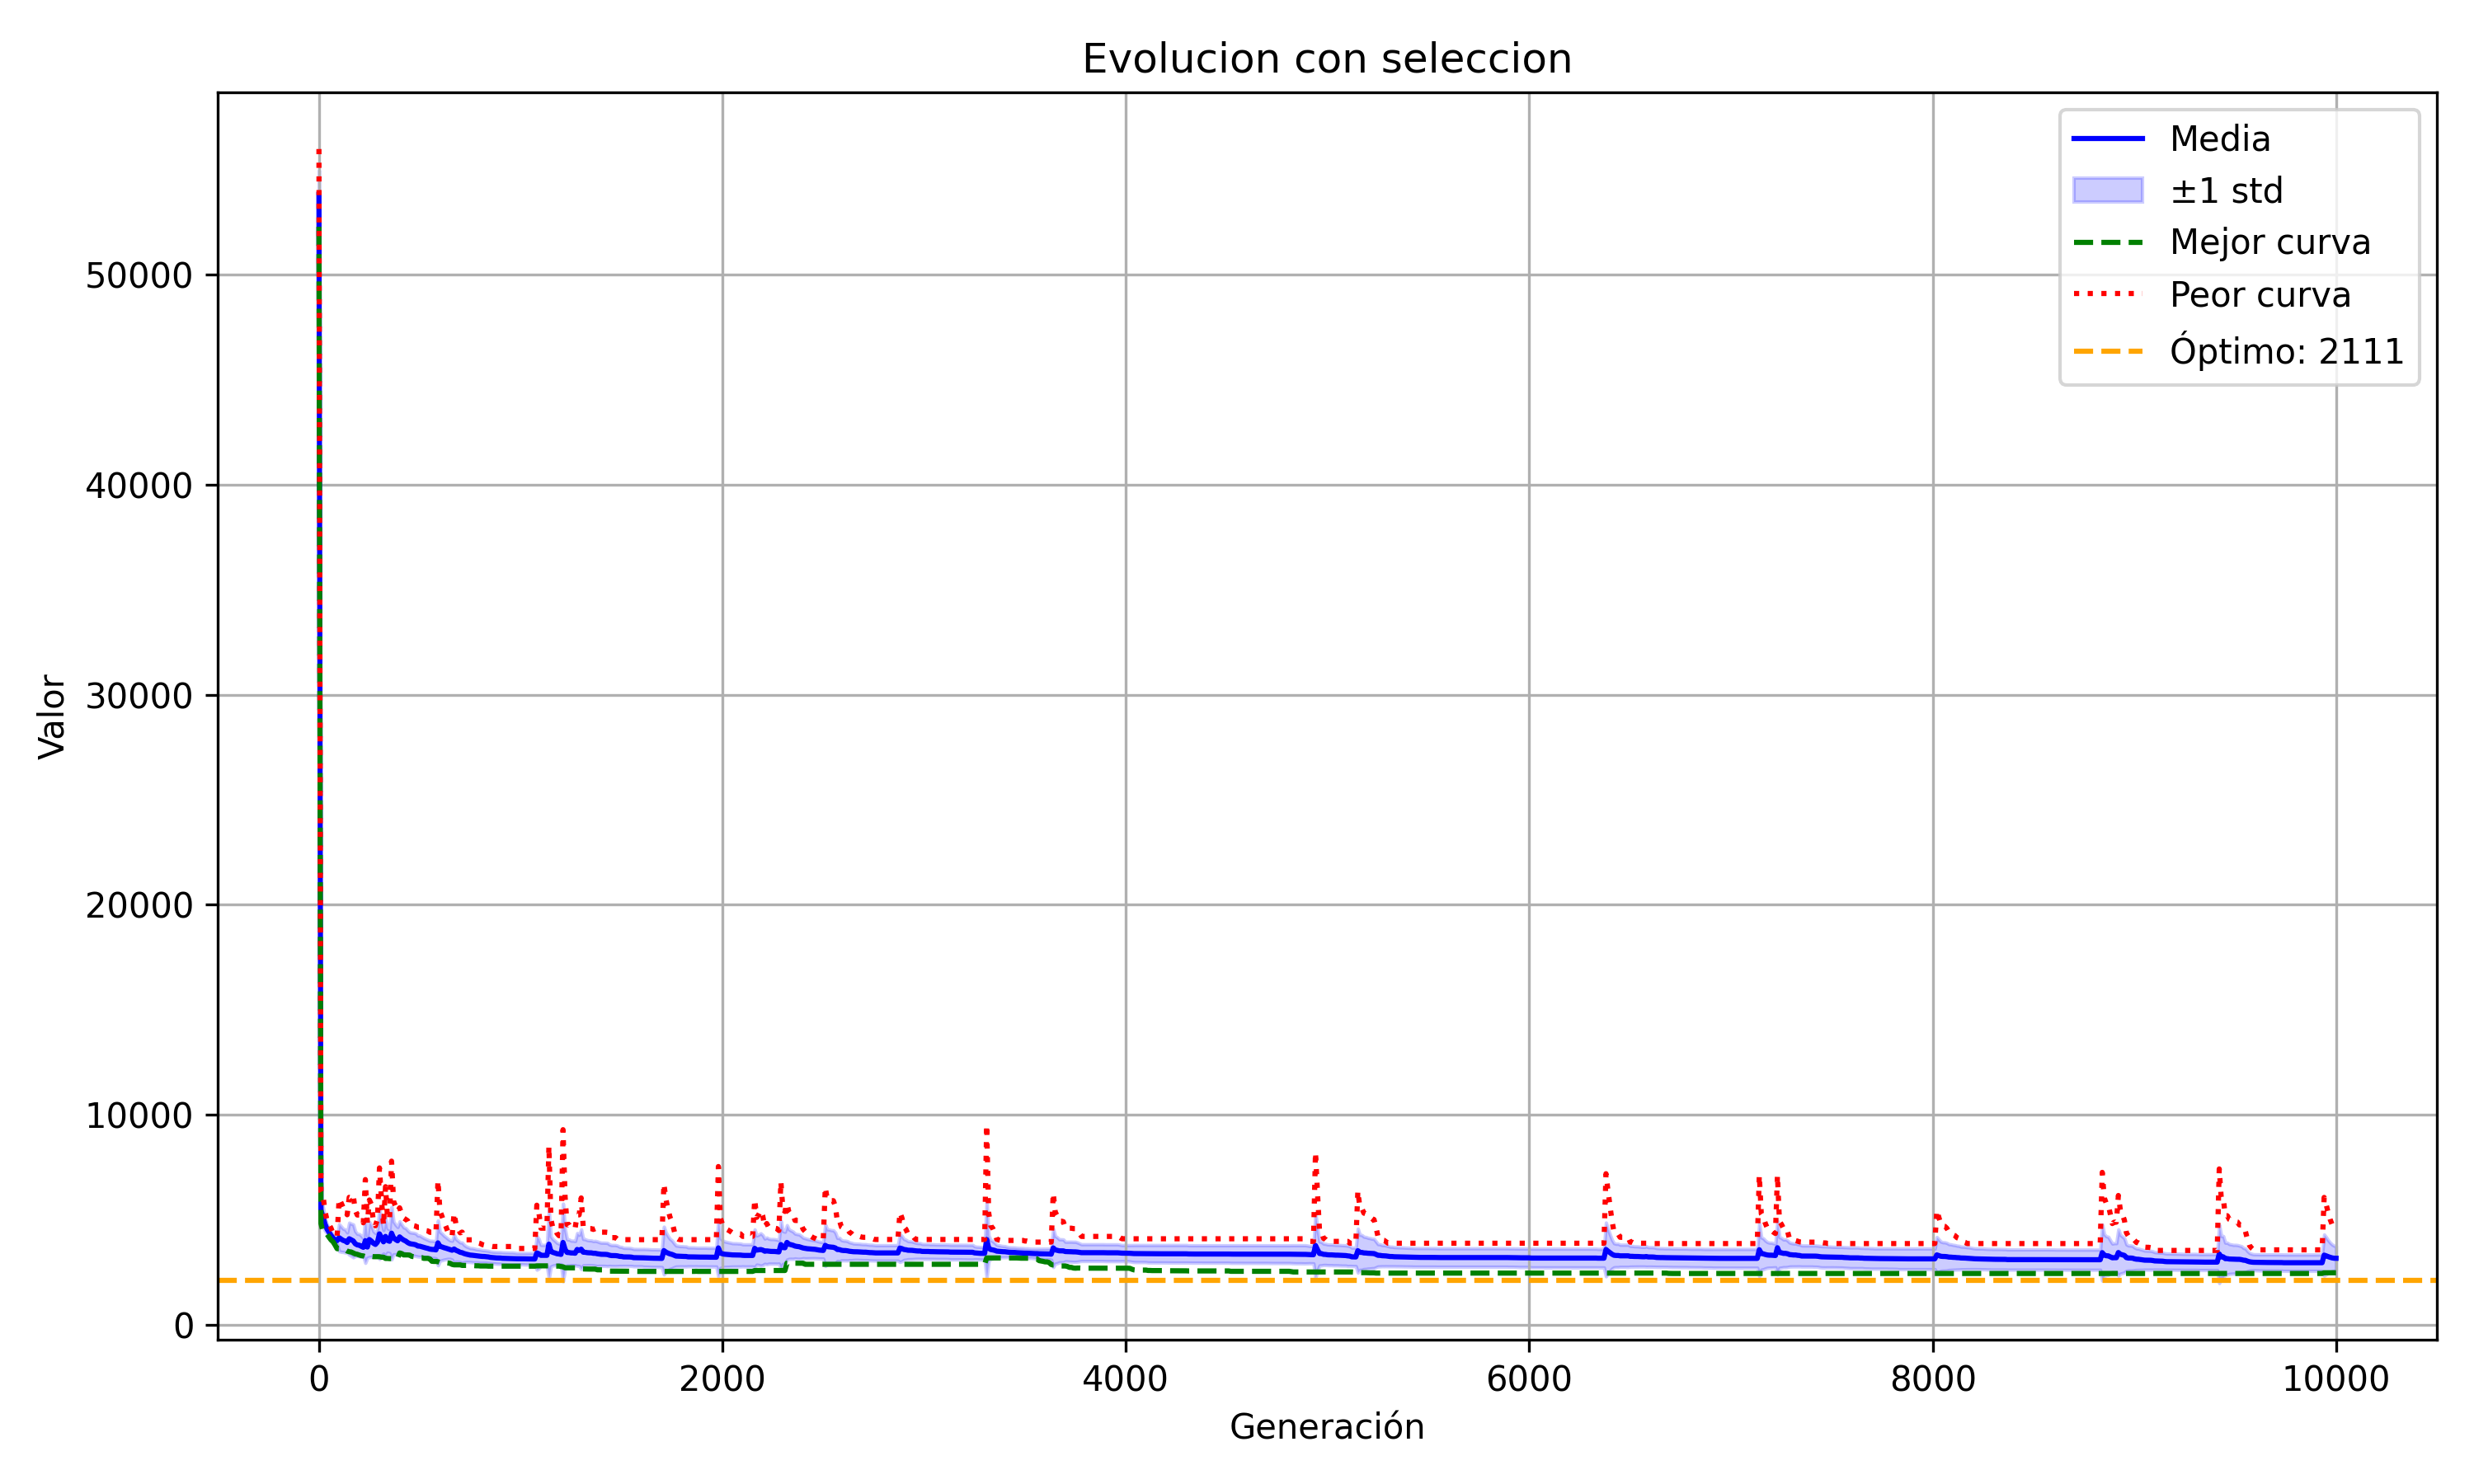
\includegraphics[width=\linewidth]{DATA/scholl_M33.png}
        \caption{Gráfico sobre las soluciones de Scholl con numero de estaciones, $m=33$}
        \label{fig:evolucion-punt}
\end{figure}
Para este grafo en particular, nuestra mejor solución alcanzó un tiempo máximo de $2440$, frente al óptimo conocido de $2111$. Si bien no se llegó al valor óptimo, lo realmente destacable es que esta solución fue encontrada tras explorar únicamente un $1{,}379 \cdot 10^{-36}\%$ del espacio total de soluciones. Esto refleja la eficiencia del algoritmo genético a la hora de identificar soluciones cercanas al óptimo sin recurrir a una exploración exhaustiva del espacio de búsqueda. 
Otros resultados donde el, $\%$ de error indica el error respecto a la solución exacta:
\begin{table}[H]
    \centering
    
    \label{tab:otros-resultados}
    \begin{tabular}{|c|c|c|c|c|c|}
        \hline
        \textbf{Grafo} & $\mathbf{m}$ & \textbf{dim\_Pobl} & \textbf{num\_Gen} & \textbf{\% Error} & \textbf{\% del espacio explorado} \\
        \hline
        BUXEY      & 10 & 500 & 500  & 0.00\%  & 1.3 \\
        LUTZ1      & 8  & 500 & 1000 & 0.00\%  & 2.4 \\
        LUTZ2      & 15 & 100 & 1000 & 5.90\%  & $1.3 \cdot 10^{-9}$ \\
        WEE-MAG    & 7  & 500 & 1000 & 0.47\%  & 0.03 \\
        WARNECKE   & 10 & 500 & 1000 & 3.90\%  & $1.0 \cdot 10^{-5}$ \\
        TONGE      & 7  & 500 & 1000 & 0.80\%  & $4.7 \cdot 10^{-4}$ \\
        TONGE      & 10 & 500 & 2000 & 2.30\%  & $2.5 \cdot 10^{-6}$ \\
        BATHOLD    & 5  & 500 & 500  & 0.27\%  & 0.51 \\
        KILBRID    & 9  & 500 & 1000 & 1.60\%  & 0.056 \\
        GUNTHER    & 10 & 500 & 500  & 4.00\%  & 0.14 \\
        \hline
    \end{tabular}
    \caption{Resumen de resultados destacables en diferentes grafos.}
\end{table}

\section{Conclusión}

El uso de algoritmos genéticos para modelizar el problema SALBP-2 demostró ser eficaz en la generación de soluciones cercanas al óptimo. Gracias a este trabajo hemos podido profundizar en como modelizar usando este tipo de algoritmos, en que centrarse para hacerlos mas eficaces, así como aprovechar toda la información que tenemos acerca de las condiciones del problema para poder modelizarlo de una manera mas sencilla como son el caso de usar el orden topológico y la uniformidad de las poblaciones iniciales.

\end{document}
